
\section{图表展示}
% 子图展示示例
\begin{frame}
\frametitle{子图展示示例}
\begin{figure}
\centering
\subfloat[子图A]{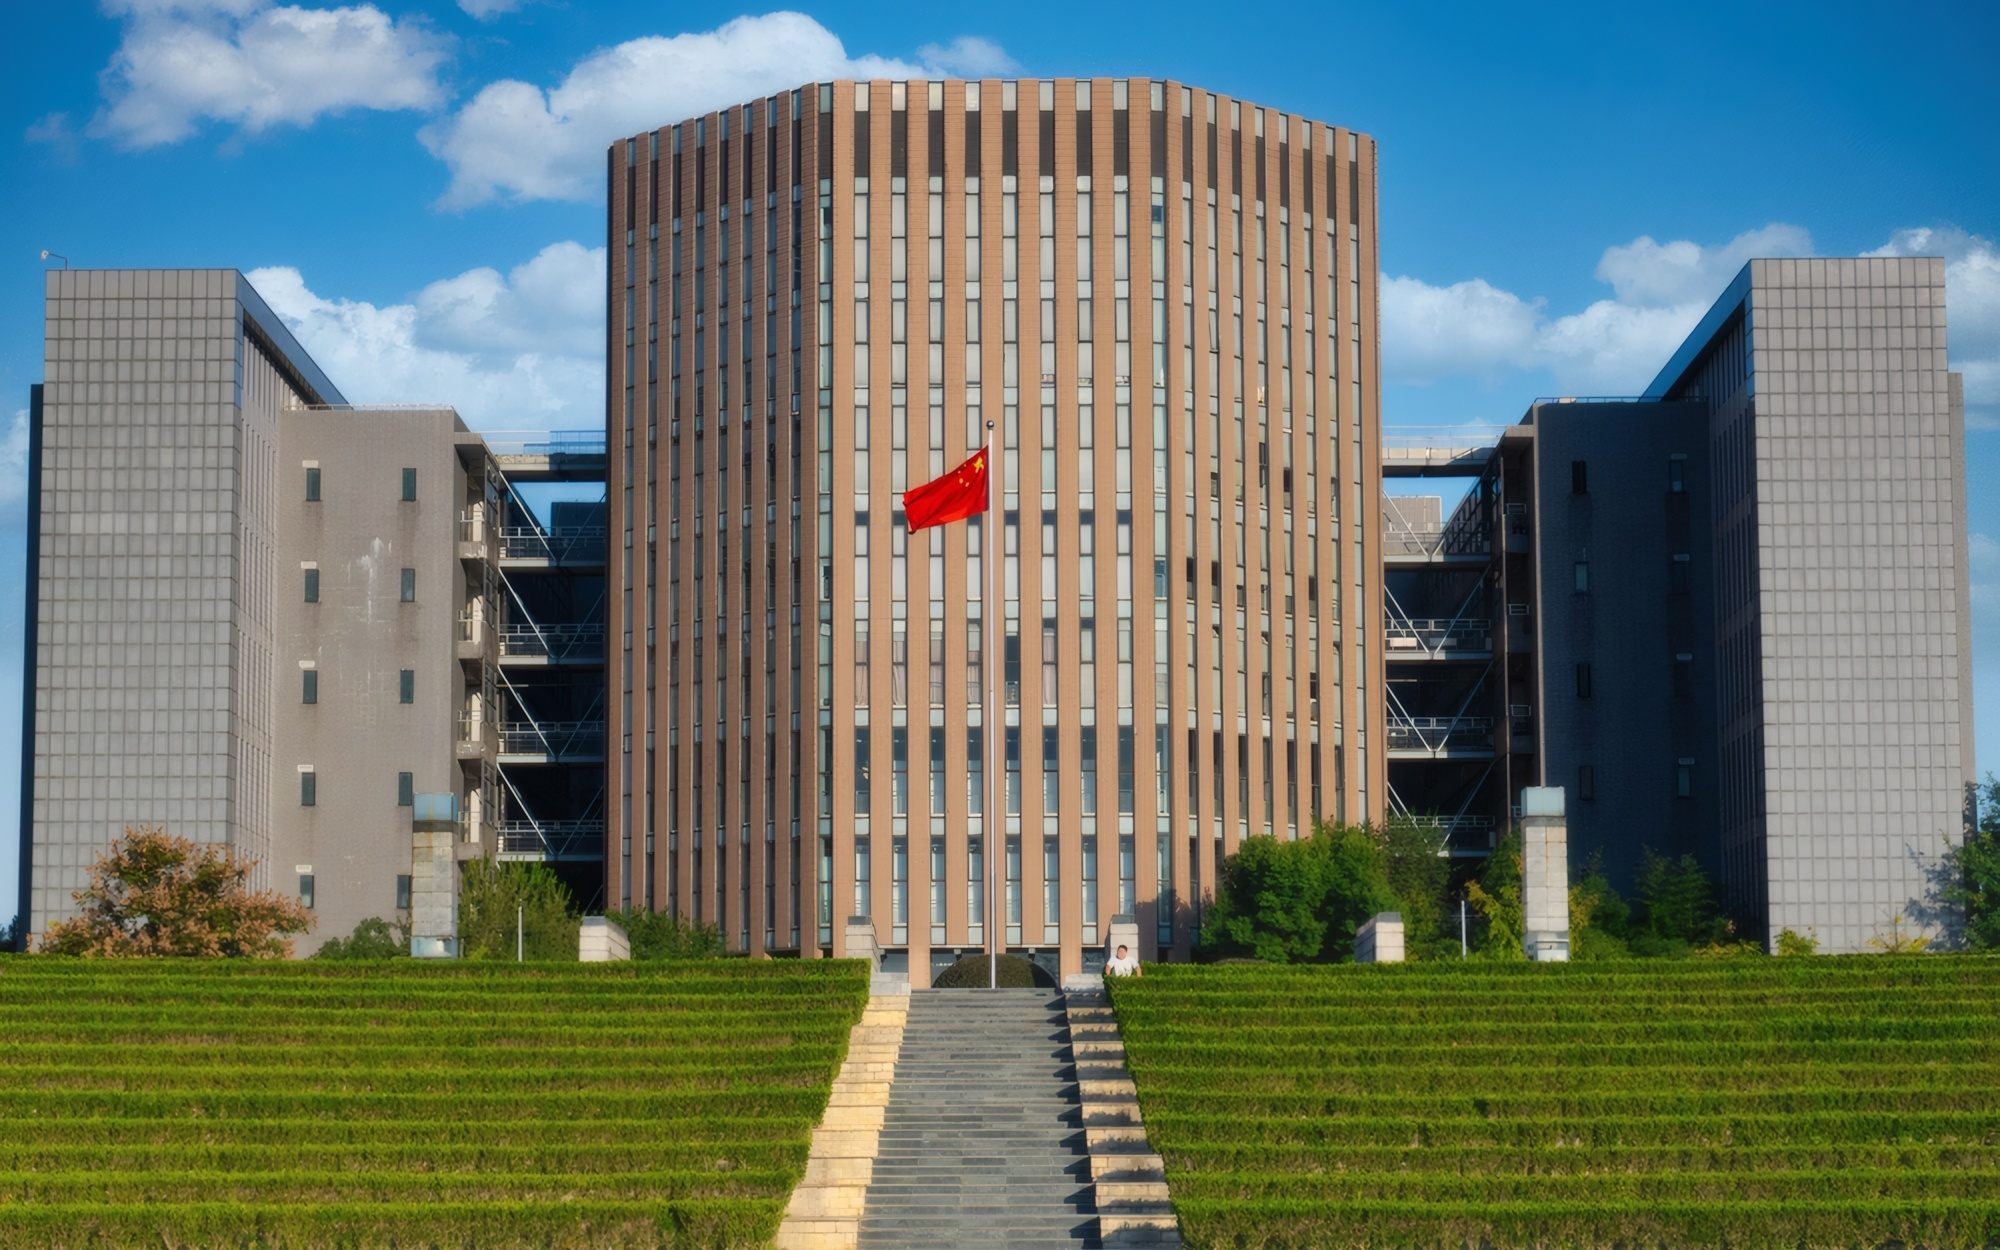
\includegraphics[width=0.45\linewidth]{src/example_ahu.jpg}\label{fig:subfig-a}}
\hfill
\subfloat[子图B]{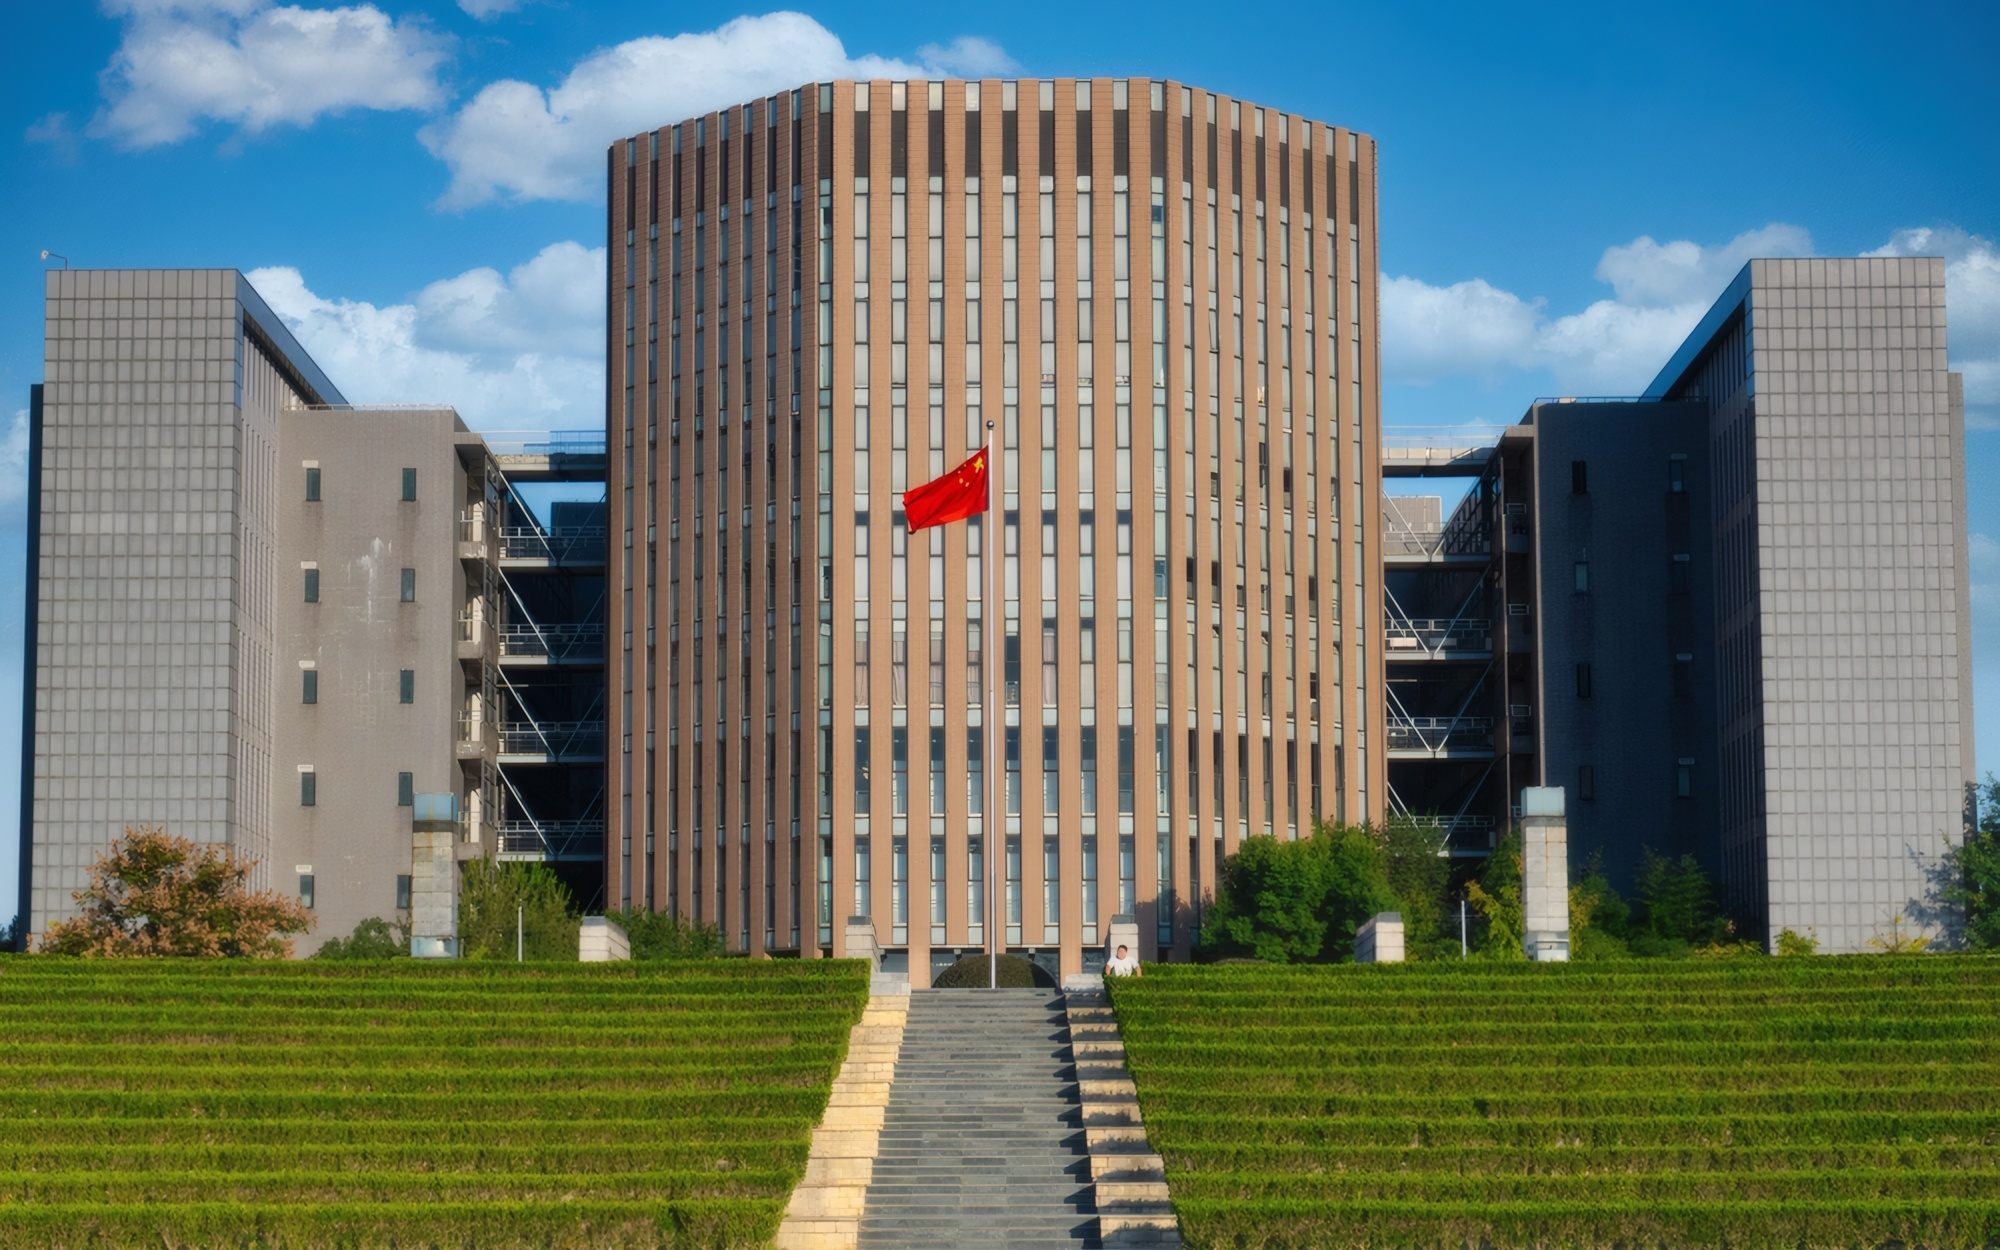
\includegraphics[width=0.45\linewidth]{src/example_ahu.jpg}\label{fig:subfig-b}}
\caption{两个并排的子图示例}
\label{fig:subfigures}
\end{figure}
这是对子图内容的简要描述。
\end{frame}

% 表格展示示例
\begin{frame}
\frametitle{表格展示示例}

\begin{table}[H]
\caption{\textbf{Example 4}}
\centering
\begin{tabular}{cccc}
\toprule
&\multicolumn{2}{c}{Resultsummary}& \\
Item1&Item2&Item3&Item4 \\
\midrule 
Data1&Data2&Data3&Data4 \\
\midrule
Data5&Data6&Data7&Data8 \\
\bottomrule
\end{tabular}
\end{table}


这是对表格内容的简要描述。
\end{frame}

% TikZ绘图示例
\begin{frame}
\frametitle{TikZ绘图示例}
\begin{figure}
\centering
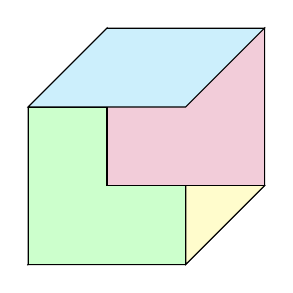
\begin{tikzpicture}[x={(1cm,0cm)}, y={(0.5cm,0.5cm)}, z={(0cm,1cm)}]
  % 绘制立方体
  \draw[fill=blue!20] (0,0,0) -- (2,0,0) -- (2,2,0) -- (0,2,0) -- cycle;
  \draw[fill=red!20] (0,0,0) -- (0,0,2) -- (0,2,2) -- (0,2,0) -- cycle;
  \draw[fill=green!20] (0,0,0) -- (2,0,0) -- (2,0,2) -- (0,0,2) -- cycle;
  \draw[fill=yellow!20] (2,0,0) -- (2,2,0) -- (2,2,2) -- (2,0,2) -- cycle;
  \draw[fill=purple!20] (0,2,0) -- (2,2,0) -- (2,2,2) -- (0,2,2) -- cycle;
  \draw[fill=cyan!20] (0,0,2) -- (2,0,2) -- (2,2,2) -- (0,2,2) -- cycle;
\end{tikzpicture}
\caption{TikZ绘制的示例图形}
\end{figure}
这是对TikZ绘图的简要描述。
\end{frame}